\section{Generative Pipeline for \dataset{}}
\label{sec:dataset}


\begin{figure*}[t]
    \centering
    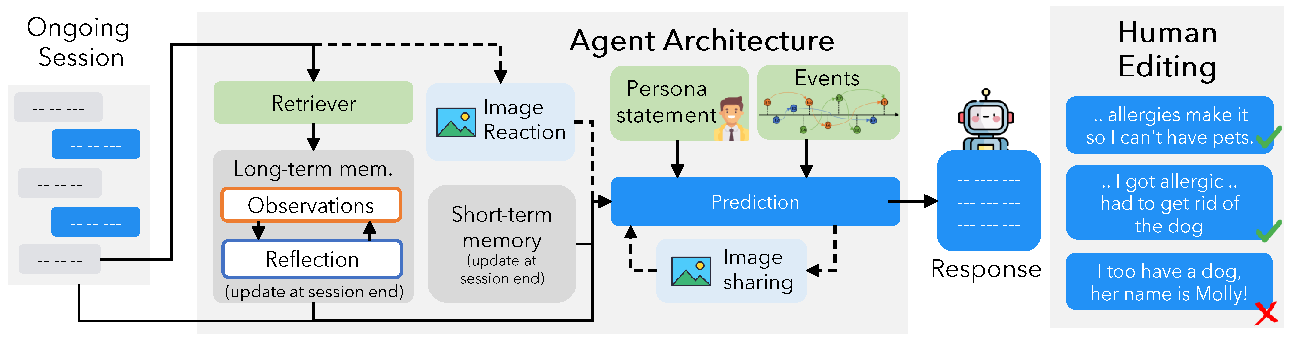
\includegraphics[width=0.99\textwidth]{figures/main_v4.pdf}
    \vspace{-1pt}
    \caption{\textbf{Overview of the generative pipeline for \dataset{}.} Each LLM agent is assigned a distinct persona and a timeline of causally connected events in their file. The agent is equipped with a memory and reflection module to retrieve relevant history for dialog generation and is also enabled for image-sharing and image-reaction behaviors (left). The generated conversations are edited by human annotators to maintain long-range consistency (right).}
    \label{fig:main}
    \vspace{-1pt}
\end{figure*}


An overview of our generative pipeline for \dataset{} is shown in Figure~\ref{fig:main}.
We create two virtual agents, 
named $\mathcal{L}_1$ and $\mathcal{L}_2$, each initialized with a LLM $\mathcal{M}$ (\textit{i.e.,} \texttt{gpt-3.5-turbo}).
To start, unique persona statements $p$ are assigned to each agent $\mathcal{L}_i$, ensuring the integration of distinct personalities into their dialogues (\Sref{ssec:dataset-persona}).
To mirror real-life experiences, we create a temporal event graph $\mathcal{G}$ for each agent, which illustrates a realistic sequence of life events (\Sref{ssec:temporal-event}).
The LLM agent architecture~\cite{park2023generative} is utilized for each agent $\mathcal{L}_i$, enabling them to effectively memorize and reflect conversation history into ongoing dialogues (\Sref{ssec:llm-agent}).
Further, each agent $\mathcal{L}_i$ can share coherent images, thereby enhancing the multi-modal dialogue aspect.
Finally, human annotators are tasked with manually filtering and refining the generated data (\Sref{ssec:manual-filter}).
%See an overview in Figure~\ref{fig:main}.

\subsection{Persona} 
\label{ssec:dataset-persona}
We select an initial persona statement $p_c$ from the MSC dataset~\cite{xu2022beyond}, encompassing 4 to 5 sentences, 
and employ \texttt{gpt-3.5-turbo} as $\mathcal{M}$ to expand these into full persona statement $p$ (See examples and prompt details in Appendix~\ref{ssec:persona_appendix}). The generated statements typically include details about one or more of the following elements~\cite{gao2023peacok}: objectives, past experiences, daily habits, and interpersonal relationships, as well as name, age, and gender of the individual.


\subsection{Temporal Event Graph} 
\label{ssec:temporal-event}
To utilize the real-life experiences of each agent in the conversation, we construct a temporal event graph, labeled as $\mathcal{G}$, for each agent. 
This graph $\mathcal{G}$, consisting of events $e_{i}$, is produced by applying the condition of $\mathcal{M}$ (i.e., \texttt{text-davinci-003}) on a designated persona $p$. Each event $e_{i}$ is associated with a date of occurrence $t_{i}$.
$\mathcal{G}$ includes causal connections $l = (e_i, e_j)$ that illustrate the causal relationships among events $e_i \in \mathcal{G}$ and reflect a natural succession of events in an individual's life. For each $\mathcal{G}$, we create up to 25 events, spread across a time frame of 6 to 12 months, in an iterative process that balances between inference time and the coherence of temporal and causal connections in the timeline. Initially, a small batch of $k=3$ events is generated, which is then used iteratively as input prompt to create the subsequent batch of $k$ events. See details in Appendix~\ref{ssec:event_appendix}.




\subsection{Virtual Agent Architecture}
\label{ssec:llm-agent}
Every agent $\mathcal{L}_i$  incorporates modules from generative agent architecture~\cite{park2023generative}.
The agent has two functions: (1) \textit{reflect \& respond}; and (2) \textit{image sharing \& image reaction}.
The agent is asked to primarily use the \textit{reflect \& respond} function while employing \textit{image sharing \& image reaction} function judiciously and appropriately within the context of the conversation.


\paragraph{Reflect \& Respond.}
The fundamental process for each agent to \textit{reflect and respond} involves the concept of short-term and long-term memory.
During inference, agent $\mathcal{L}_i$ conditions its responses on both short and long-term memories, paralleling how humans remember recent conversations while also recalling distilled important experiences from long-term memory. Following each session $k$, each agent is asked to produce a summary $w_k$ that is then stored in the short-term $\mathcal{H}_s$. This summary $w_k$ is generated by conditioning $\mathcal{M}$ on both the most recent session conversation history $h_{k}$ and the preceding summary $w_{k-1} \in \mathcal{H}_l$. For each turn $j$ within session $k$, a single turn of the conversation $h_{k_j}$ is transformed into an observation $o_{k_j}$ and then stored in the long-term memory $\mathcal{H}_l$. Then, agent $\mathcal{L}_i$ generates a response in session $k+1$ on the date $t_{k+1}^s$ by basing it on the latest summary $w_k$, reflections based on the retrieved relevant observations $o \in \mathcal{H}_s$, the ongoing conversation history in the current session $h_{k+1}$ and persona statement $p$. Long-term temporal narratives are induced in the conversation by additionally conditioning the agent's response on the subset of events in $\mathcal{G}$ that occur between the last and current session i.e. $\{e\in\mathcal{G}\,|\,t_{k}^s\,<\,t_{i}^e\,<\,t_{k+1}^s\,\}$. See details in Appendix~\ref{sssec:agent_appendix}.

 
\paragraph{Image Sharing \& Image Reaction.}
The \textit{image sharing \& image reaction} functions are integrated to add a multi-modal dimension to the long-term dialogues.\footnote{Image captions are also saved to long-term memory.}
The \textit{image sharing} function is called when the agent decides to send an image. This process includes:
(1) Generate a caption $c$ for the intended image using $\mathcal{M}$;
(2) Convert the caption $c$ into relevant keywords $w$ using $\mathcal{M}$;
(3) Use the keywords $k$ to find an image through web search $WEB(k)$\footnote{\url{https://pypi.org/project/icrawler/}};
(4) Share the chosen $image$.
Conversely, the \textit{image reaction} function is triggered upon receiving an image from another agent and entails:
(1) Generate caption $c$ for the received image\footnote{We use BLIP-2 \cite{li2023blip} as the captioning model.};
(2) Generate a reaction for the received image in response using $\mathcal{M}$ (See Appendix~\ref{sssec:agent_appendix}).



\subsection{Human Verification \& Editing}
\label{ssec:manual-filter}
In the concluding phase, human annotators are tasked with (1) editing the dialogue to eliminate long-term inconsistencies, (2) removing or substituting irrelevant images, and (3) verifying and editing for alignment between event graphs and the content of the conversations. Overall, we observed that annotators edited nearly 15\% of the dialog turns and removed or substituted approx. 19\% images present in the LLM-generated dataset. See examples of some edits in Appendix~\ref{ssec:edits_appendix}.
